\documentclass[a4paper]{article}
\usepackage[top=4mm, bottom=4mm, left=8mm, right=8mm]{geometry}
\usepackage{color}
\usepackage{listings}
\usepackage{mathtools}
\usepackage{amssymb}
\usepackage{graphicx}
\usepackage{float}
%\pagestyle{empty}



\title{Complexity Notes}
\date{\today}
\author{Hugo McNally}

\definecolor{comment_colour}{rgb}{0,0.6,0}
\definecolor{number_colour}{rgb}{0.5,0.5,0.5}
\definecolor{string_colour}{rgb}{0.58,0,0.82}
\lstset{
    commentstyle=\color{comment_colour},
    keywordstyle=\color{blue},
    numberstyle=\tiny\color{number_colour},
    stringstyle=\color{string_colour}
}

\begin{document}
\section*{Notes}
\begin{itemize}
    \item Learning rate of 0.05
    \item deadline of 30
    \item regular graph
    \begin{itemize}
        \item 30 nodes
        \item 5 degrees per node
    \end{itemize}
    \item trained over 10,000 episodes
    \item tested over 1,000 episodes
\end{itemize}

\begin{figure}
\centering
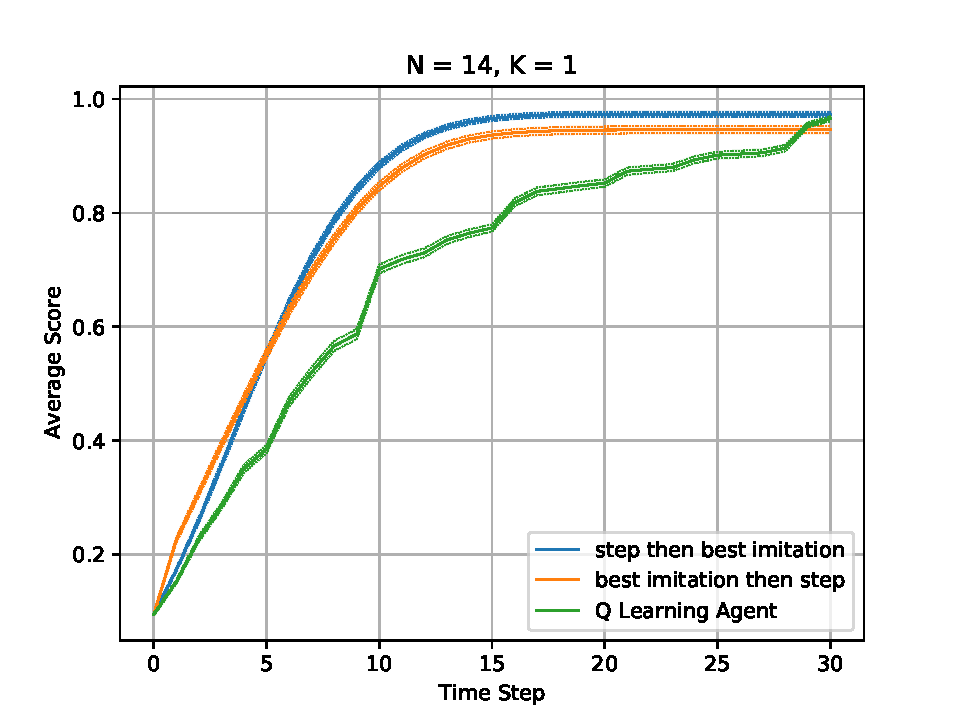
\includegraphics[width=30em]{../figures/comp1.pdf}
\caption{
    Heuristic approaches compared a Q-learning approach,
    with an NK landscape of N = 14 and K = 1.
}
\label{comp1}
\end{figure}

\begin{figure}
\centering
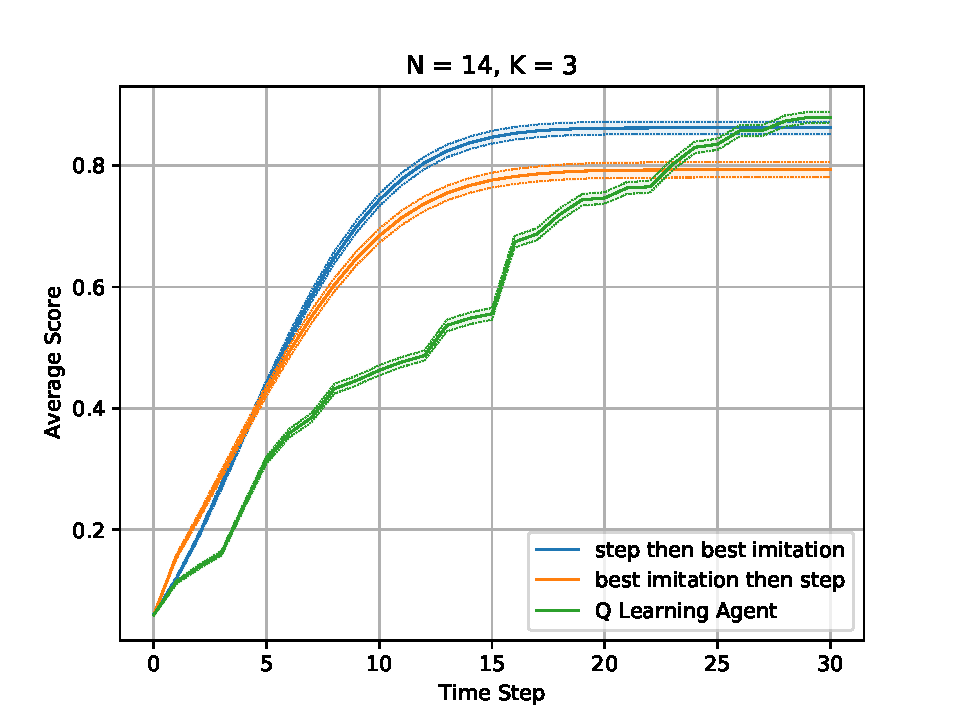
\includegraphics[width=30em]{../figures/comp3.pdf}
\caption{
    Heuristic approaches compared a Q-learning approach,
    with an NK landscape of N = 14 and K = 3.
}
\label{comp3}
\end{figure}

\begin{figure}
\centering
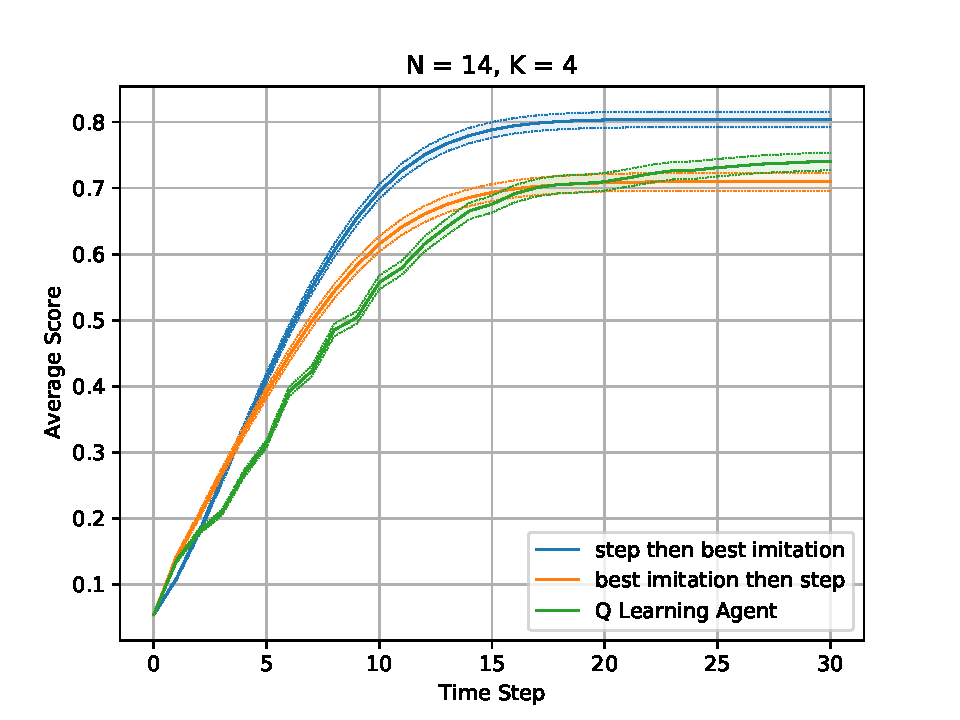
\includegraphics[width=30em]{../figures/comp4.pdf}
\caption{
    Heuristic approaches compared a Q-learning approach,
    with an NK landscape of N = 14 and K = 4.
}
\label{comp4}
\end{figure}

\begin{figure}
\centering
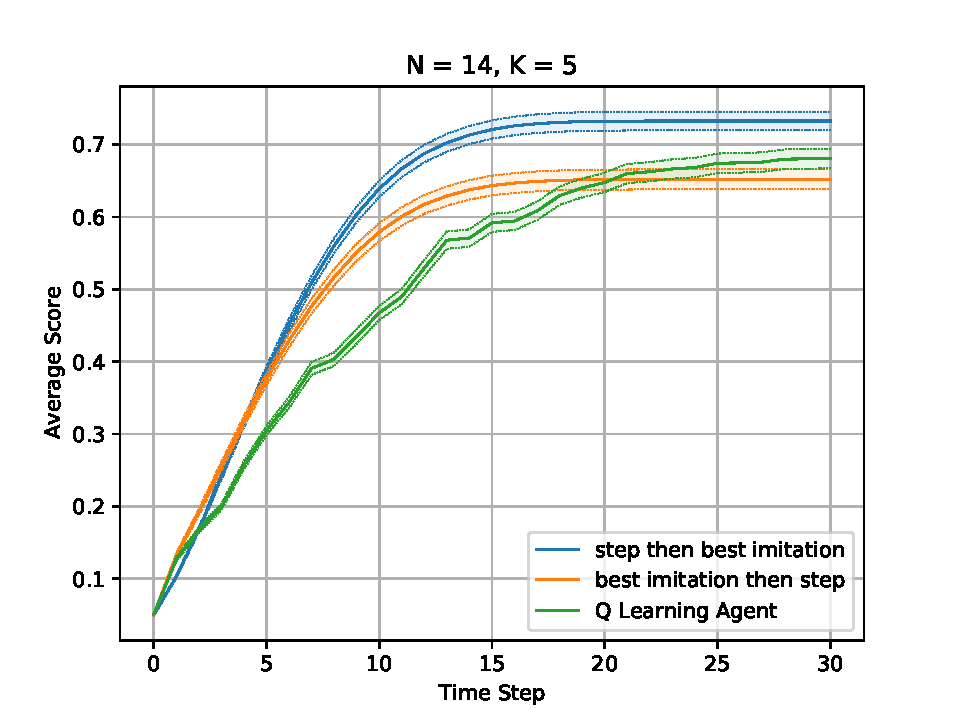
\includegraphics[width=30em]{../figures/comp5.pdf}
\caption{
    Heuristic approaches compared a Q-learning approach,
    with an NK landscape of N = 14 and K = 5.
}
\label{comp5}
\end{figure}

\begin{figure}
\centering
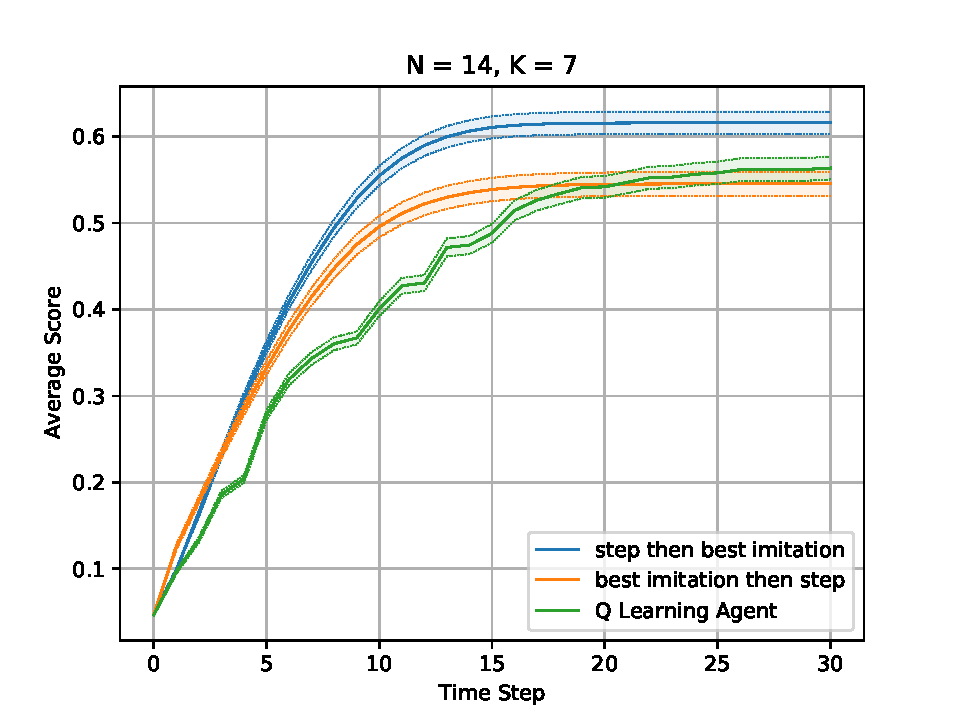
\includegraphics[width=30em]{../figures/comp7.pdf}
\caption{
    Heuristic approaches compared a Q-learning approach,
    with an NK landscape of N = 14 and K = 7.
}
\label{comp7}
\end{figure}

\begin{figure}
\centering
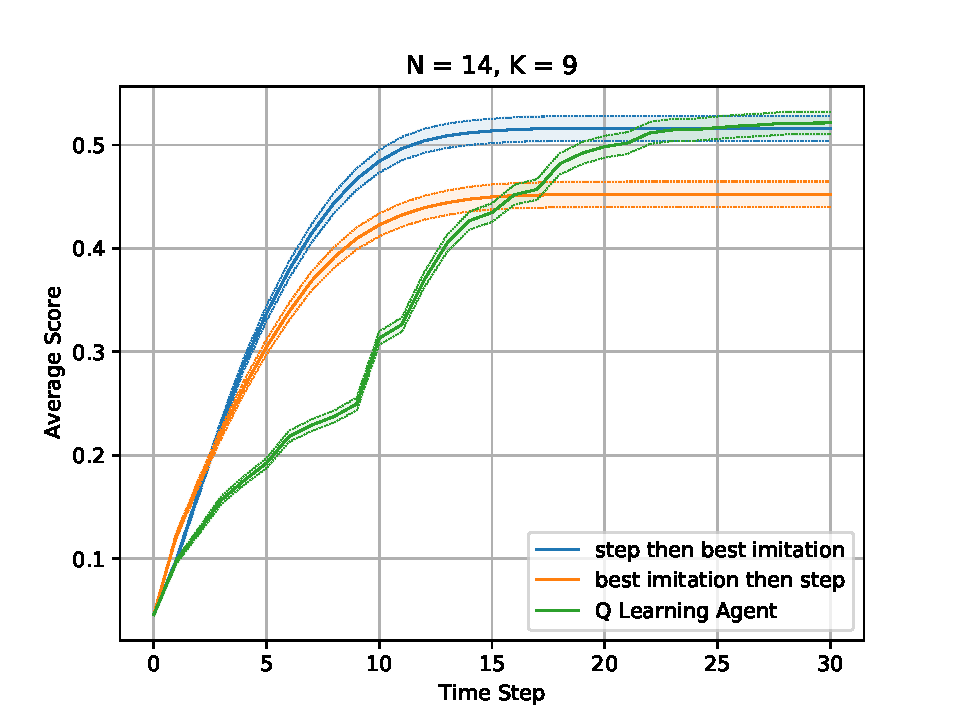
\includegraphics[width=30em]{../figures/comp9.pdf}
\caption{
    Heuristic approaches compared a Q-learning approach,
    with an NK landscape of N = 14 and K = 9.
}
\label{comp9}
\end{figure}

\begin{figure}
\centering
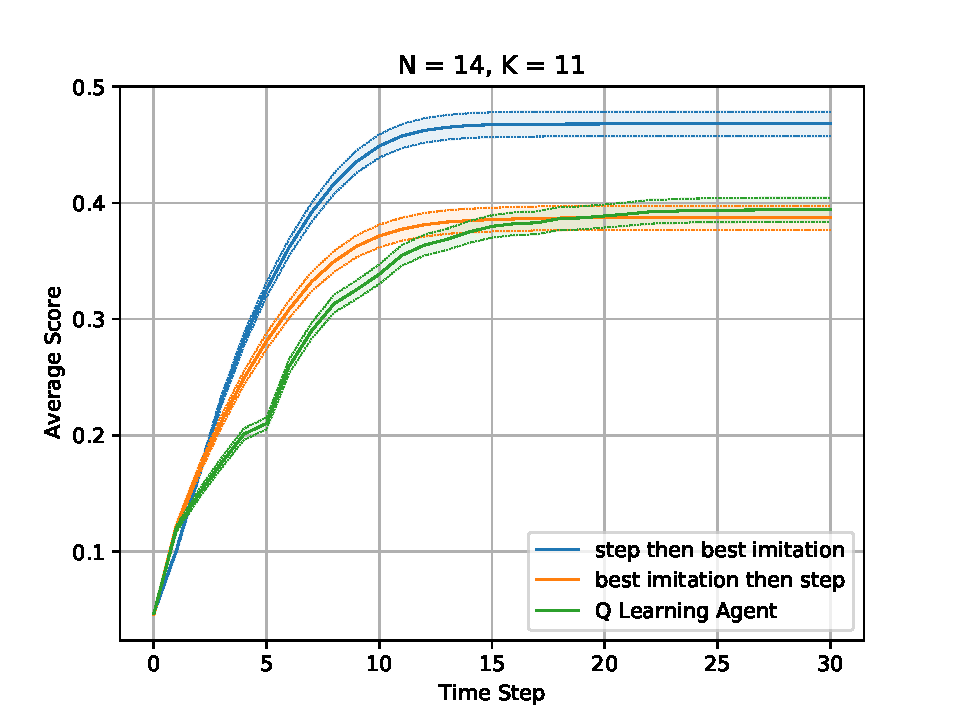
\includegraphics[width=30em]{../figures/comp11.pdf}
\caption{
    Heuristic approaches compared a Q-learning approach,
    with an NK landscape of N = 14 and K = 11.
}
\label{comp11}
\end{figure}

\end{document}
